\documentclass{article}

% Pacotes extras necessários
\usepackage{amsmath}
\usepackage[lmargin=0.7in, rmargin=0.7in, tmargin=0.5in, bmargin=0.5in, includehead, includefoot]{geometry}
\usepackage{amsfonts}
\usepackage[utf8]{inputenc}
\usepackage[portuguese]{babel}
\usepackage{graphicx}
\usepackage{fancyhdr}
\usepackage{setspace}

\graphicspath{ {./images/} }

% Sets para outras partes
\setlength{\parindent}{0pt}
\setstretch{1.25}
\DeclareMathOperator{\sen}{sen}

% ------- Estilo do trabalho -------- %
\fancypagestyle{capa}{
    \fancyhf{}
    \renewcommand\headrulewidth{0pt}
    \fancyfoot[C]{
        Rio de Janeiro\\
        2022
    }
}

\pagestyle{fancy}
\fancyhead{}
\fancyhead[L]{\thepage}
\fancyfoot{}
% ----------------------------------- %

% Dados do Grupo
\title{Sinais e Sistemas - Trabalho 3 - Avaliação 5}
\author{
    \textbf{Grupo 2}\\
    Leonardo Soares da Costa Tanaka\\
    Matheus Henrique Sant Anna Cardoso\\
    Theo Rudra Macedo e Silva
}
\date{}


\begin{document}

% Capa
\maketitle
\thispagestyle{capa}

\newpage

\textbf{1.)} Um SLIT é modelado por $\tau \dot{y}(t) + y(t) = u(t)$ com $y(0^{-}) = \alpha$.
\textbf{G2:} $\tau = 3, \alpha = -2$

\textbf{(a)} Calcular a resposta ao degrau unitário e esboçar o seu gráfico;

Para calcular a resposta, trataremos já com os dados, sendo a EDO:
\[3\dot{y}(t) + y(t) = 1(t)\,\,\,\,,\,\,\,\,y(0^{-}) = -2\]
Pela propriedade da derivação, sabemos que
\[\dot{y}(t) = sY(s) - y(0^{-})\]
Então
\begin{align*}
    \mathcal{L}\{3\dot{y}(t) + y(t)\} &= \mathcal{L}\{u(t)\}\\
    3(sY(s) - y(0^-)) + Y(s) &= U(s)\\
    Y(s)(3s + 1) + 6 &= U(s)
\end{align*}

Como $u(t) = 1(t)$, sabemos que $U(s) = \frac{1}{s}$, assim

\begin{align*}
    Y(s)(3s + 1) + 6 = \frac{1}{s}\\
    Y(s) = \frac{1}{3s + 1} \cdot \frac{1}{s} - \frac{6}{3s + 1}
\end{align*}

Separando em frações parciais, temos:

\begin{align*}
    Y(s) &= \frac{1}{s} - \frac{3}{3s + 1} - \frac{6}{3s + 1}\\
    Y(s) &= \frac{1}{s} - \frac{9}{3s + 1}\\
    Y(s) &= \frac{1}{s} - \frac{3}{s + 1/3}
\end{align*}

Agora, podemos descobrir $y(t)$.

\begin{align*}
    \mathcal{L}^{-1} \biggl\{\frac{1}{s}\biggr\} &= 1(t) & \mathcal{L}^{-1}\biggl\{\frac{3}{s + 1/3}\biggr\} &= 3e^{-\frac{1}{3}t}1(t)
\end{align*}

\begin{align*}
    \mathcal{L}^{-1} \left\{Y(s)\right\} &= 1(t) - 3e^{-\frac{1}{3}t}1(t)
\end{align*}

Finalmente

\[y(t) = 1(t) - 3e^{-\frac{t}{3}}1(t)\]

\newpage

\begin{figure}[h]
    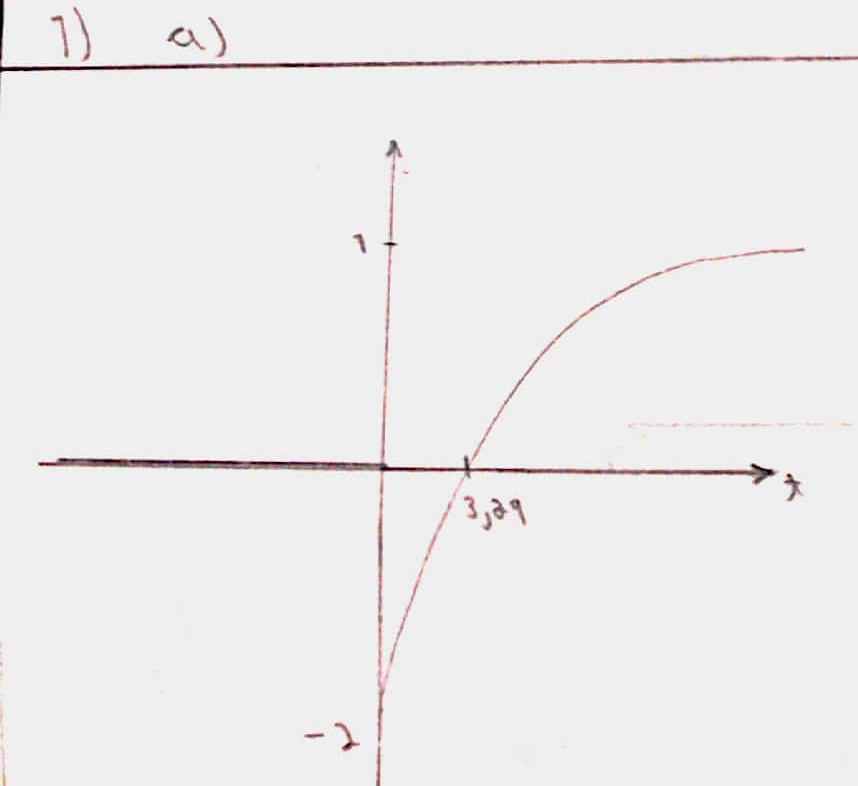
\includegraphics[scale=0.25]{Q1_a.png}
    \centering
    \caption{Esboço do gráfico - Questão 1) a)}
\end{figure}

\textbf{(b)} calcular a resposta à rampa unitária e esboçar o seu gráfico;

Para calcular a resposta à rampa, tomemos a seguinte EDO:

\[3\dot{y}(t) + y(t) = t1(t) \,\,\,\,,\,\,\,\,y(0^-) = -2\]

Da mesma forma como no item \textbf{(a)}, podemos utilizar a propriedade da derivação e fazer em ambos os lados, a transformada de Laplace.

\begin{align*}
    \mathcal{L}\left\{\dot{y}(t)\right\} &= \left(sY(s) - y(0^-)\right) & \mathcal{L}\left\{t1(t)\right\} = U(s) &= \frac{1}{s^2}
\end{align*}
\begin{align*}
    3(Y(s) - y(0^-)) + Y(s) = U(s)\\
    Y(s)(3s + 1) + 6 = \frac{1}{s^2}\\
    Y(s) = \frac{1}{3s + 1}\cdot\frac{1}{s^2} - \frac{6}{3s + 1}
\end{align*}

Separando em frações parciais, teremos

\begin{align*}
    Y(s) &= \frac{9}{3s + 1} - \frac{3s - 1}{s^2} - \frac{6}{3s + 1}\\
    Y(s) &= \frac{3}{3s + 1} - \frac{3s - 1}{s^2}\\
    Y(s) &= \frac{1}{s + 1/3} - \frac{3}{s} + \frac{1}{s^2}
\end{align*}

Agora, podemos calcular a inversa da transformada de Laplace.

\begin{align*}
    \mathcal{L}^{-1} \left\{\frac{1}{s + 1/3}\right\} &= e^{-\frac{t}{3}}1(t) & \mathcal{L}^{-1} \left\{\frac{3}{s}\right\} &= 3\cdot1(t) & \mathcal{L}^{-1} \left\{\frac{1}{s^2}\right\} &= t1(t)\\
\end{align*}
\begin{align*}
    \mathcal{L}^{-1} \left\{Y(s)\right\} &= e^{-\frac{t}{3}}1(t) - 3\cdot1(t) + t1(t)
\end{align*}
Finalmente
\[y(t) = e^{-\frac{t}{3}}1(t) - 3\cdot1(t) + t1(t)\]

\begin{figure}[h]
    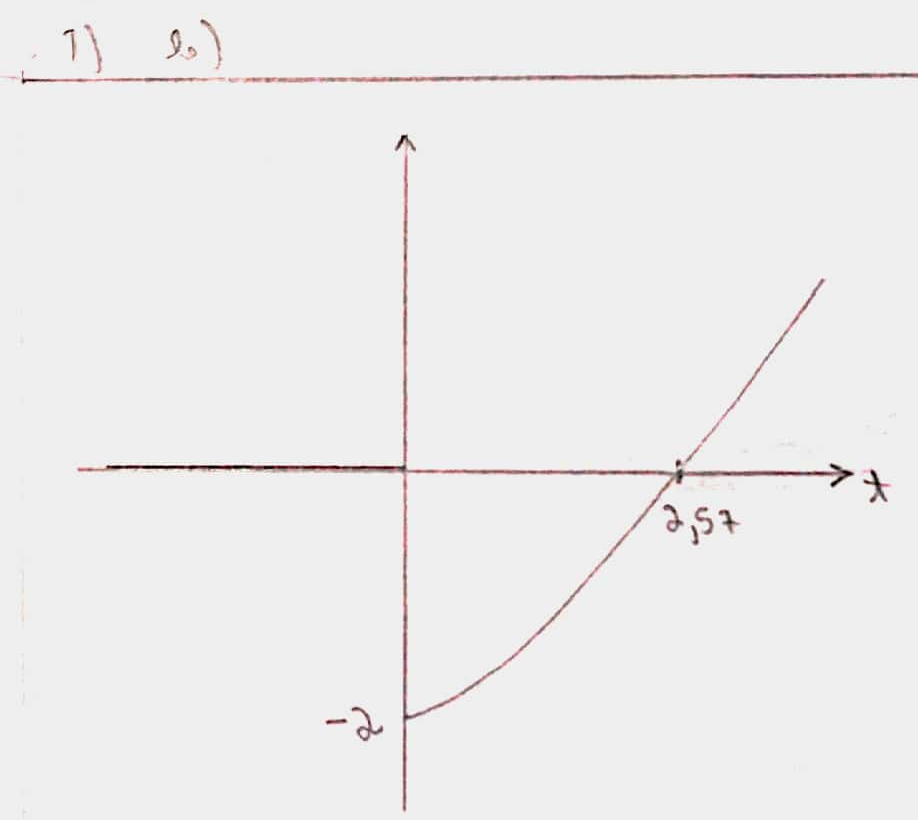
\includegraphics[scale=0.25]{Q1_b.png}
    \centering
    \caption{Esboço do gráfico - Questão 1) b)}
\end{figure}

\textbf{(c)} calcular a resposta ao seno $u(t) = \sen(\omega t)$ para $\alpha = 0,\, \omega = 1/(4\tau)$ e esboçar o seu gráfico;

Agora, temos para resolver a seguinte EDO:

\[ 3\dot{y}(t) + y(t) = \sen\left(\frac{t}{12}\right)1(t) \,\,\,\,,\,\,\,\, y(0^-) = 0\]

Utilizaremos Laplace, para resolver, a saber

\begin{align*}
    \mathcal{L}\left\{\dot{y}(t)\right\} &= sY(s) & \mathcal{L}\left\{\sen \left(\frac{t}{12}1(t)\right) \right\} &= \frac{1/12}{s^2 + 1 / 144} = \frac{12}{144s^2 + 1}
\end{align*}

Utilizando, novamente, as técnicas empregadas nos itens anteriores, teremos

\begin{align*}
    3(sY(s)) + Y(s) = \frac{12}{144s^2 + 1}\\
    Y(s)(3s + 1) = \frac{12}{144s^2 + 1}\\
    Y(s) = \frac{1}{3s + 1} \cdot \frac{12}{144s^2 + 1}\\
    Y(s) = \frac{r_1}{3s + 1} + \frac{r_2}{144s^2 + 1}
\end{align*}

Vamos, por tentativa e erro, calcular as constantes $r_1 \text{ e } r_2$.

Perceba que, fazendo $r_1 \cdot (144s^2 + 1)$ teremos um termo com $s^2$ mais uma constante. O mesmo deve ser para $r_2 \cdot (3s + 1)$. Para isso, podemos fazer com que o segundo seja o produto da soma pela diferença, obtendo um termo ao quadrado e uma constante.

Fazemos, então $r_2 = (3s - 1)$, obtendo, naquele segundo produto, o seguinte: $r_2 \cdot (3s + 1) = (3s - 1) (3s + 1) = 9s^2 - 1$.

No primeiro produto ($r_1 \cdot (144s^2 + 1)$), já temos um fator grande suficiente para o termo quadrático, podemos corrigir com o segundo produto, multiplicando por 16.

No final, ficamos com a expressão

\[\frac{1}{3s + 1} - \frac{16(3s - 1)}{144s^2 + 1}\]

Ficamos, porém, com uma constante no numerador igual a ($144s^2 + 1 - 16(9s^2 - 1) = 1 + 16 = 17$) diferente da expressão original ($12$). Sendo assim, podemos multiplicar a expressão toda por $\frac{12}{17}$ para termos a expressão inicial na forma de somas parciais.

Então

\[Y(s) = \left(\frac{1}{3s + 1} - \frac{16(3s - 1)}{144s^2 + 1}\right) \cdot \frac{12}{17}\]

Assim

\[Y(s) \cdot \frac{17}{12} = \frac{1}{3s + 1} - \frac{48s - 16}{144s^2 + 1}\]

Fazendo mais alterações, teremos

\begin{align*}
    Y(s) \cdot \frac{17}{12} = \frac{1}{3s + 1} - \frac{48s}{144s^2 + 1} + \frac{16}{144s^2 + 1}\\
    Y(s) \cdot \frac{17}{12} = \frac{1/3}{s + 1/3} - \frac{1}{3}\cdot\frac{s}{s^2 + 1/144} + \frac{4}{3}\cdot\frac{1/12}{s^2 + 1/144}
\end{align*}

\begin{align*}
    \mathcal{L}^{-1} \left\{\frac{1}{s + 1/3}\right\} &= e^{-\frac{t}{3}}1(t) & \mathcal{L}^{-1} \left\{\frac{s}{s^2 + 1/144}\right\} &= \cos\left(\frac{t}{12}\right)1(t) & \mathcal{L}^{-1} \left\{\frac{1/12}{s^2 + 1/144}\right\} &= \sen\left(\frac{t}{12}\right)1(t)
\end{align*}

\begin{align*}
    \mathcal{L}^{-1} \left\{Y(s) \cdot \frac{17}{12}\right\} = \frac{e^{-\frac{t}{3}}1(t)}{3} - \frac{\cos\left(\frac{t}{12}\right)1(t)}{3} + \frac{4}{3}\cdot sen\left(\frac{t}{12}\right)1(t)\\
    y(t) \cdot \frac{17}{4} = e^{-\frac{t}{3}}1(t) - \cos\left(\frac{t}{12}\right)1(t) + 4sen\left(\frac{t}{12}\right)1(t)\\
\end{align*}

Finalmente

\[y(t) = 1(t)\cdot\frac{4e^{-\frac{t}{3}} - 4\cos\left(\frac{t}{12}\right) + 16sen\left(\frac{t}{12}\right)}{17}\]

\begin{figure}[h!]
    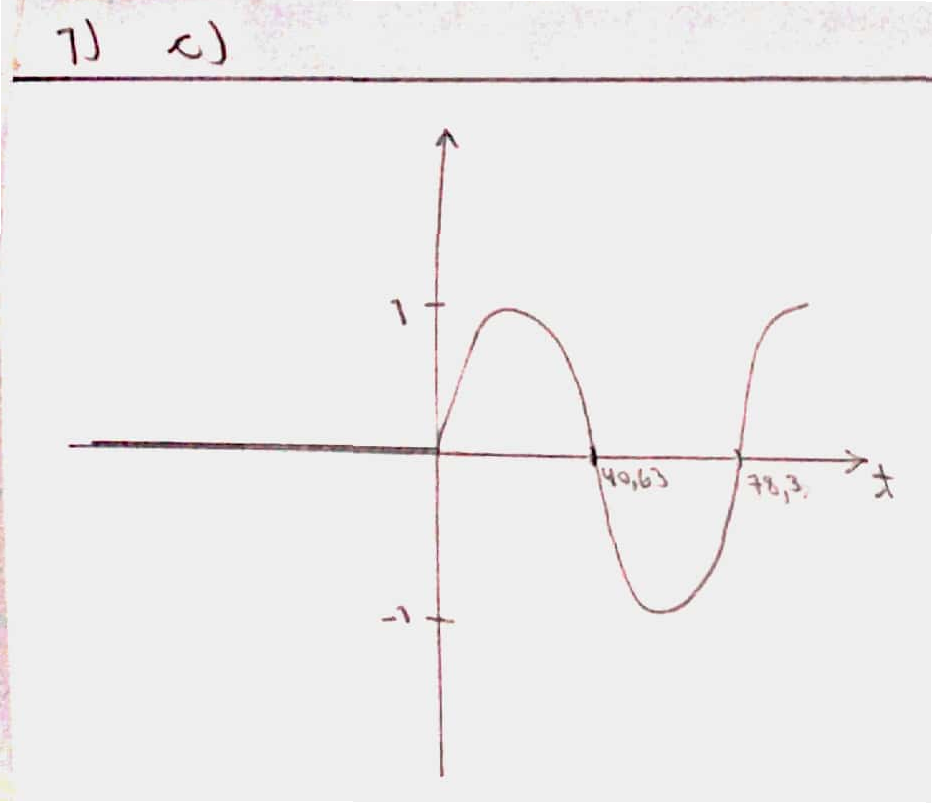
\includegraphics[scale=0.25]{Q1_c.png}
    \centering
    \caption{Esboço do gráfico - Questão 1) c)}
\end{figure}

\textbf{(d)} calcular a resposta ao seno $u(t) = \sen(\omega t)$ para $\alpha = 0,\, \omega = 4/\tau$ e esboçar o seu gráfico;

Agora, temos para resolver a seguinte EDO:

\[ 3\dot{y}(t) + y(t) = \sen\left(\frac{4t}{3}\right)1(t) \,\,\,\,,\,\,\,\, y(0^-) = 0\]

Utilizaremos Laplace, para resolver, a saber

\begin{align*}
    \mathcal{L}\left\{\dot{y}(t)\right\} &= sY(s) & \mathcal{L}\left\{\sen \left(\frac{4t}{3}1(t)\right) \right\} &= \frac{4/3}{s^2 + 16/9} = \frac{12}{9s^2 + 16}
\end{align*}

Utilizando, novamente, as técnicas empregadas nos itens anteriores, teremos

\begin{align*}
    3(sY(s)) + Y(s) = \frac{12}{9s^2 + 16}\\
    Y(s)(3s + 1) = \frac{12}{9s^2 + 16}\\
    Y(s) = \frac{1}{3s + 1} \cdot \frac{12}{9s^2 + 16}\\
    Y(s) = \frac{r_1}{3s + 1} + \frac{r_2}{9s^2 + 16}
\end{align*}

Vamos, por tentativa e erro, calcular as constantes $r_1 \text{ e } r_2$.

Perceba que, fazendo $r_1 \cdot (9s^2 + 16)$ teremos um termo com $s^2$ mais uma constante. O mesmo deve ser para $r_2 \cdot (3s + 1)$. Para isso, podemos fazer com que o segundo seja o produto da soma pela diferença, obtendo um termo ao quadrado e uma constante.

Fazemos, então $r_2 = (3s - 1)$, obtendo, naquele segundo produto, o seguinte: $r_2 \cdot (3s + 1) = (3s - 1) (3s + 1) = 9s^2 - 1$.

No primeiro produto ($r_1 \cdot (9s^2 + 16)$), já temos um fator multiplicado pelo termo quadrático, igual ao outro. Não tendo a necessidade de multiplicarmos por nada. Assim, ficamos com $r_1 = 1$.

No final, ficamos com a expressão

\[\frac{1}{3s + 1} - \frac{(3s - 1)}{9s^2 + 16}\]

Ficamos, porém, com uma constante no numerador igual a ($9s^2 + 16 - (9s^2 - 1) = 16 + 1 = 17$) diferente da expressão original ($12$). Sendo assim, podemos multiplicar a expressão toda por $\frac{12}{17}$ para termos a expressão inicial na forma de somas parciais.

Então

\[Y(s) = \left(\frac{1}{3s + 1} - \frac{3s - 1}{9s^2 + 16}\right) \cdot \frac{12}{17}\]

Assim

\[Y(s) \cdot \frac{17}{12} = \frac{1}{3s + 1} - \frac{3s - 1}{9s^2 + 16}\]

Fazendo mais alterações, teremos

\begin{align*}
    Y(s) \cdot \frac{17}{12} = \frac{1}{3s + 1} - \frac{3s}{9s^2 + 16} + \frac{1}{9s^2 + 16}\\
    Y(s) \cdot \frac{17}{12} = \frac{1/3}{s + 1/3} - \frac{1}{3}\cdot\frac{s}{s^2 + 16/9} + \frac{1}{12}\cdot\frac{4/3}{s^2 + 16/9}
\end{align*}

\begin{align*}
    \mathcal{L}^{-1} \left\{\frac{1}{s + 1/3}\right\} &= e^{-\frac{t}{3}}1(t) & \mathcal{L}^{-1} \left\{\frac{s}{s^2 + 1/144}\right\} &= \cos\left(\frac{t}{12}\right)1(t) & \mathcal{L}^{-1} \left\{\frac{1/12}{s^2 + 1/144}\right\} &= \sen\left(\frac{t}{12}\right)1(t)
\end{align*}

\begin{align*}
    \mathcal{L}^{-1} \left\{Y(s) \cdot \frac{17}{12}\right\} = \frac{e^{-\frac{t}{3}}1(t)}{3} - \frac{\cos\left(\frac{4t}{3}\right)1(t)}{3} + \frac{1}{12}\cdot sen\left(\frac{4t}{3}\right)1(t)\\
    y(t) \cdot 17 = 4e^{-\frac{t}{3}}1(t) - 4\cos\left(\frac{4t}{3}\right)1(t) + sen\left(\frac{t}{12}\right)1(t)\\
\end{align*}

Finalmente

\[y(t) = 1(t)\cdot\frac{4e^{-\frac{t}{3}} - 4\cos\left(\frac{4t}{3}\right) + sen\left(\frac{4t}{3}\right)}{17}\]

\begin{figure}[h]
    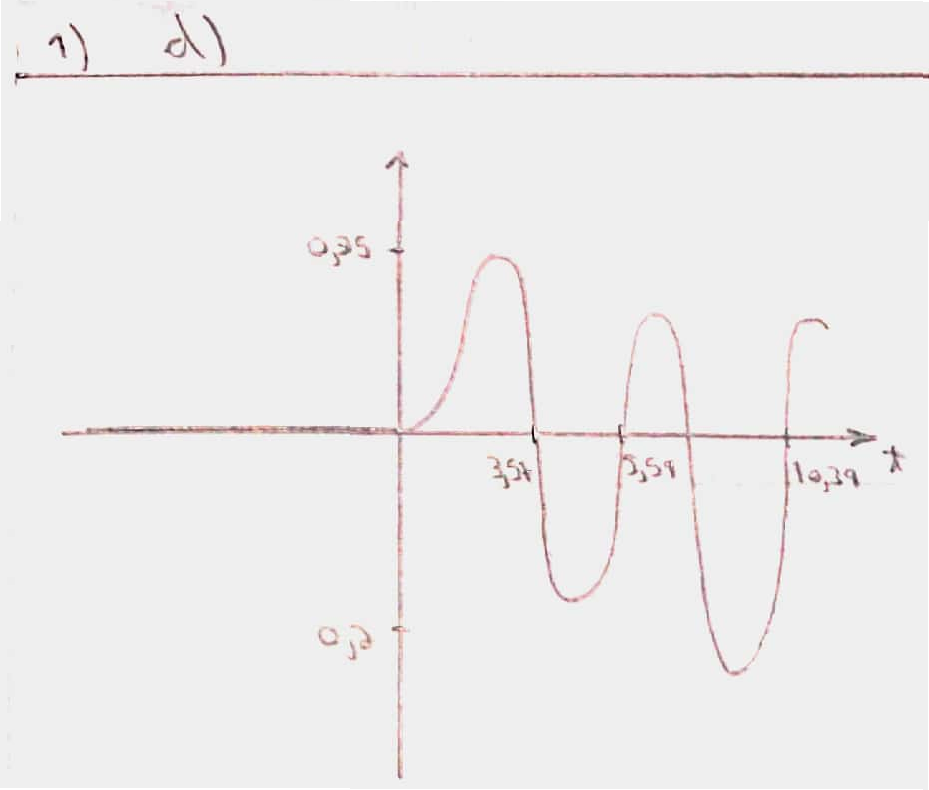
\includegraphics[scale=0.25]{Q1_d.png}
    \centering
    \caption{Esboço do gráfico - Questão 1) d)}
\end{figure}

\textbf{(e)} encontrar a entrada $u(t)$ para que $y(t) = \alpha\,\forall t \geq 0$;

Trabalhando com a seguinte EDO, teremos:

\[3\dot{y}(t) + y(t) = u(t)\,\,\,\,,\,\,\,\,y(0^-) = -2\]

Porém, temos que $y(t) = -2 \forall t \geq 0$. Assim, podemos definir a função $y(t) = -2$, pois respeitará o fato de $y(0^-) = -2$. Dessa forma, $\dot{y}(t) = 0$. Na equação, teremos:

\[3\cdot 0 + (-2) = u(t)\]
Finalmente
\[u(t) = -2\]

\textbf{(f)} encontrar a entrada $u(t)$ para que  $y(t) = 0\,\forall t > 0$.

Aqui, devemos tomar o cuidado para manter a condição de que $y(0^-) = -2$. Para isso, podemos definir que
\[y(t) = -2 \cdot 1(-t)\]
Tendo, por consequência que
\[\dot{y}(t) = -2\delta(-t) = -2\delta(t)\]
Acima, utilizamos a inversão na escala de tempo para chegar que $\dot{y}(t) = -2\delta(t)$.

Agora, podemos resolver a equação, que é dada por

\[3\dot{y}(t) + y(t) = u(t)\,\,\,\,,\,\,\,\,y(0^-) = -2\]
\[3(-2\delta(t)) + (-2\cdot 1(t)) = u(t)\]
Finalmente
\[u(t) = -6\delta(t) - 2\cdot 1(t)\]

\vspace{\baselineskip}

\textbf{2.)} Um SLIT relaxado é descrito por $\ddot{y}(t) + a_1\dot{y}(t) + a_0y(t) = b_1\dot{u}(t) + u(t)$.
\textbf{G2:} $a_1 = 30, a_0 = 3$

\textbf{(a)} Para $b_1 = 0$ calcular a resposta ao degrau unitário e esboçar o seu gráfico;

\[\ddot{y}(t) + 30\dot{y}(t) + 3y(t) = u(t)\,\,\,\,,\,\,\,\,y(0^{-}) = 0\]

\[\mathcal{L} \left\{\ddot{y}(t) + 30\dot{y}(t) + 3y(t)\right\} = \mathcal{L} \left\{1(t)\right\}\]

\[ s^{2}Y(s) + 30sY(s) + 3Y(s) = \frac{1}{s} \]

\[ Y(s) = \frac{1}{s \cdot (s^{2} + 30s + 3)} = \frac{1}{s} \cdot \frac{1}{(s + 15 - \sqrt{222}) \cdot (s + 15 + \sqrt{222})} =\]

\[ = \frac{1}{s} \cdot \left(\frac{ \frac{\sqrt{222}}{444}}{s + 15 - \sqrt{222}} - \frac{\frac{\sqrt{222}}{444}}{s + 15 + \sqrt{222}}\right) \]

\[ y(t) = \int \mathcal{L}^{-1} \left\{\frac{\sqrt{222}}{444} \cdot \left[ \frac{1}{s + 15 - \sqrt{222}} - \frac{1}{s + 15 + \sqrt{222}} \right] \right\} = \]

\[ = \frac{\sqrt{222}}{444} \cdot \int (e^{(-15+\sqrt{222})t} - e^{(-15-\sqrt{222})t}) dt = \frac{\sqrt{222}}{444} \cdot \left\{ \frac{e^{(-15+\sqrt{222})t}}{-15+\sqrt{222}} - \frac{e^{(-15-\sqrt{222})t}}{-15-\sqrt{222}} \right\}  \]

\begin{figure}[h]
    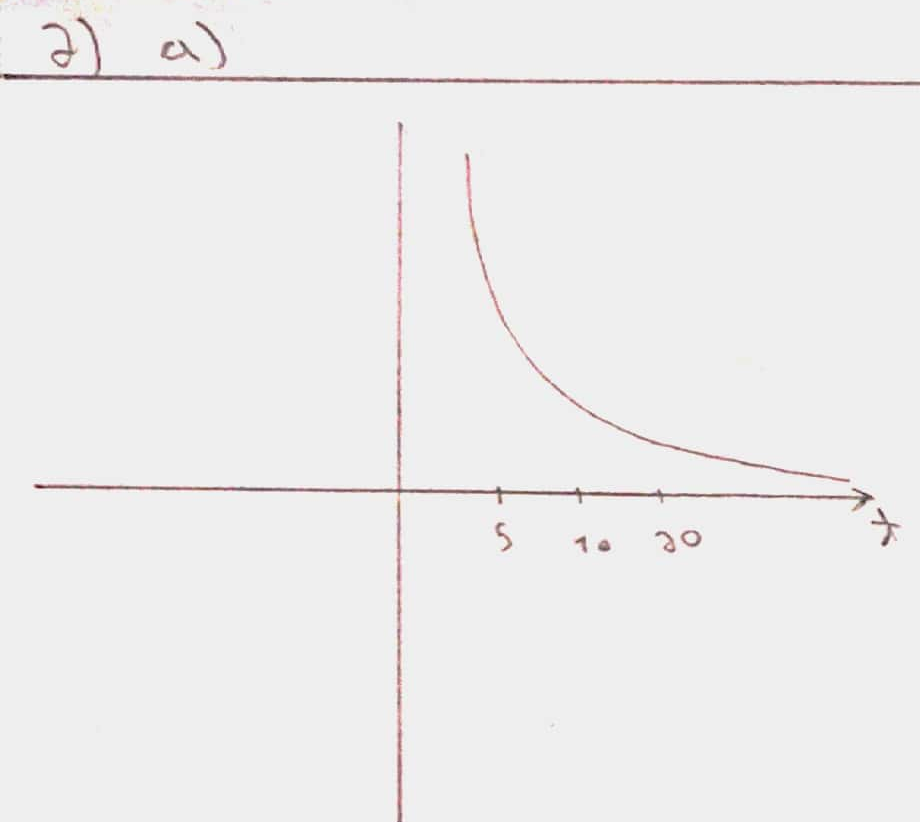
\includegraphics[scale=0.25]{Q2_a.png}
    \centering
    \caption{Esboço do gráfico - Questão 2) a)}
\end{figure}

\textbf{(b)} para $b_1 = 0$ calcular a resposta à rampa unitária e esboçar o seu gráfico;

\[\ddot{y}(t) + 30\dot{y}(t) + 3y(t) = u(t)\,\,\,\,,\,\,\,\,y(0^{-}) = 0\]

\[\mathcal{L} \left\{\ddot{y}(t) + 30\dot{y}(t) + 3y(t)\right\} = \mathcal{L} \left\{t1(t)\right\}\]

\[ s^{2}Y(s) + 30sY(s) + 3Y(s) = \frac{1}{s^{2}} \]

\[ Y(s) = \frac{1}{s^{2} \cdot (s^{2} + 30s + 3)} = \frac{1}{s^{2}} \cdot \frac{1}{(s + 15 - \sqrt{222}) \cdot (s + 15 + \sqrt{222})} =\]

\[ = \frac{1}{s^{2}} \cdot \left(\frac{ \frac{\sqrt{222}}{444}}{s + 15 - \sqrt{222}} - \frac{\frac{\sqrt{222}}{444}}{s + 15 + \sqrt{222}}\right) \]

\[ y(t) = \int \int \mathcal{L}^{-1} \left\{\frac{\sqrt{222}}{444} \cdot \left[ \frac{1}{s + 15 - \sqrt{222}} - \frac{1}{s + 15 + \sqrt{222}} \right] \right\} = \]

\[ = \frac{\sqrt{222}}{444} \cdot \int \left\{ \frac{e^{(-15+\sqrt{222})t}}{-15+\sqrt{222}} - \frac{e^{(-15-\sqrt{222})t}}{-15-\sqrt{222}} \right\} dt = \frac{\sqrt{222}}{444} \cdot \left\{ \frac{e^{(-15+\sqrt{222})t}}{(-15+\sqrt{222})^{2}} - \frac{e^{(-15-\sqrt{222})}}{(-15-\sqrt{222})^{2}} \right\} \]

\begin{figure}[h]
    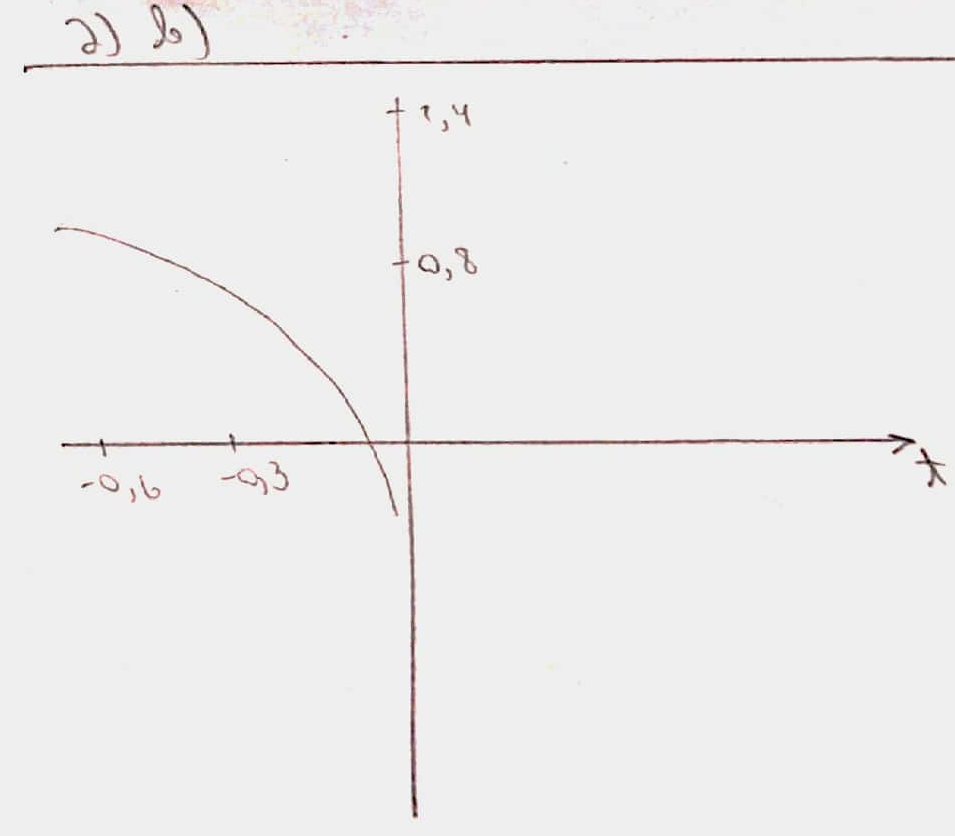
\includegraphics[scale=0.25]{Q2_b.png}
    \centering
    \caption{Esboço do gráfico - Questão 2) b)}
\end{figure}

\vspace{\baselineskip}

\textbf{(c)} para $b_1 = 1$ calcular a resposta ao degrau unitário e esboçar o seu gráfico;

\[\ddot{y}(t) + 30\dot{y}(t) + 3y(t) = \dot{u}(t) + u(t)\,\,\,\,,\,\,\,\,y(0^{-}) = 0\]

\[\mathcal{L} \left\{\ddot{y}(t) + 30\dot{y}(t) + 3y(t)\right\} = \mathcal{L} \left\{1(t) + t1(t)\right\}\]

\[ s^{2}Y(s) + 30sY(s) + 3Y(s) = 1 + \frac{1}{s} \]

\[Y(s) = \frac{1}{s^{2} + 30s + 3} + \frac{1}{s \cdot (s^{2} + 30s + 3)}\]

\[ Y(s) = \frac{1}{(s + 15 - \sqrt{222}) \cdot (s + 15 + \sqrt{222})} + \frac{1}{s} \cdot \frac{1}{(s + 15 - \sqrt{222}) \cdot (s + 15 + \sqrt{222})}\]

\[ = \frac{ \frac{\sqrt{222}}{444}}{s + 15 - \sqrt{222}} - \frac{\frac{\sqrt{222}}{444}}{s + 15 + \sqrt{222}} + \frac{1}{s} \cdot \left(\frac{ \frac{\sqrt{222}}{444}}{s + 15 - \sqrt{222}} - \frac{\frac{\sqrt{222}}{444}}{s + 15 + \sqrt{222}}\right) \]

\[ = \frac{\sqrt{222}}{444} \cdot \left\{ e^{(-15+\sqrt{222})t} - e^{(-15-\sqrt{222})t} + \frac{e^{(-15+\sqrt{222})t}}{-15+\sqrt{222}} - \frac{e^{(-15-\sqrt{222})t}}{-15-\sqrt{222}} \right\} \]

\begin{figure}[h]
    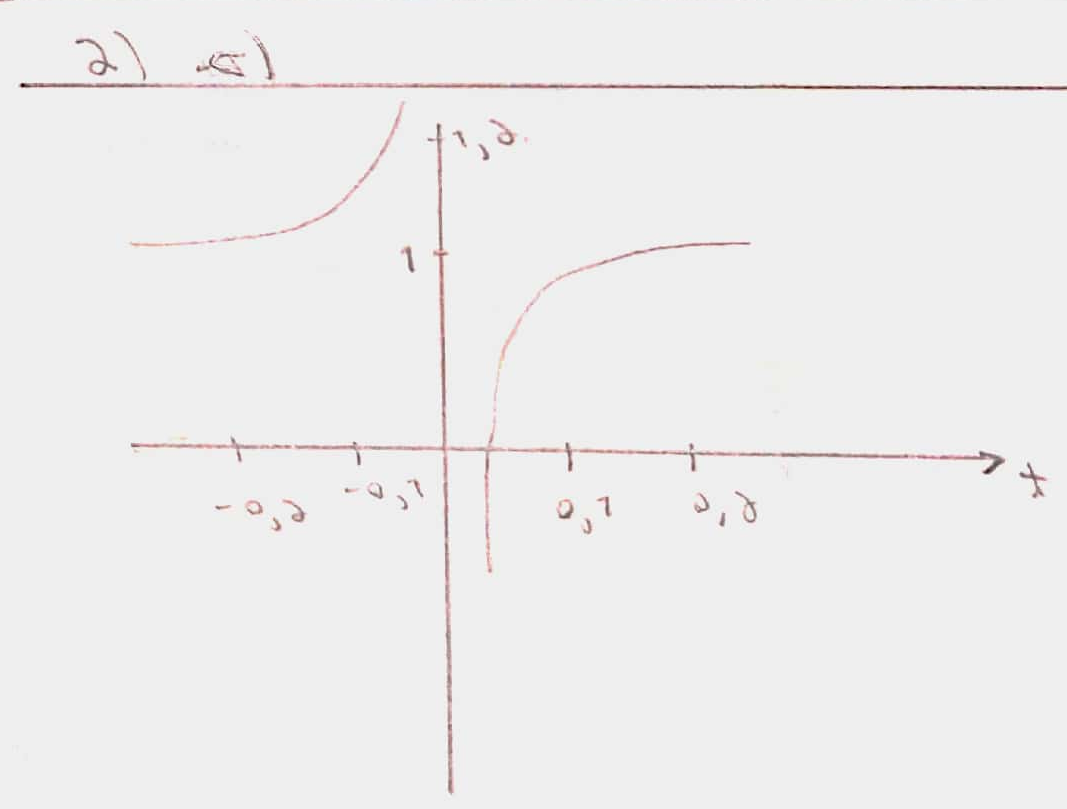
\includegraphics[scale=0.21]{Q2_c.png}
    \centering
    \caption{Esboço do gráfico - Questão 2) c)}
\end{figure}

\vspace{\baselineskip}

\textbf{(d)} para $b_1 = -1$ calcular a resposta ao degrau unitário e esboçar o seu gráfico;

\vspace{\baselineskip}

\[\ddot{y}(t) + 30\dot{y}(t) + 3y(t) = - \dot{u}(t) + u(t)\,\,\,\,,\,\,\,\,y(0^{-}) = 0\]

\[\mathcal{L} \left\{\ddot{y}(t) + 30\dot{y}(t) + 3y(t)\right\} = \mathcal{L} \left\{- 1(t) + t1(t)\right\}\]

\[ s^{2}Y(s) + 30sY(s) + 3Y(s) = - 1 + \frac{1}{s} \]

\[ Y(s) = - \frac{1}{s^{2} + 30s + 3} + \frac{1}{s \cdot (s^{2} + 30s + 3)}\]

\[ Y(s) = - \frac{1}{(s + 15 - \sqrt{222}) \cdot (s + 15 + \sqrt{222})} + \frac{1}{s} \cdot \frac{1}{(s + 15 - \sqrt{222}) \cdot (s + 15 + \sqrt{222})}\]

\[  = - \frac{ \frac{\sqrt{222}}{444}}{s + 15 - \sqrt{222}} + \frac{\frac{\sqrt{222}}{444}}{s + 15 + \sqrt{222}} + \frac{1}{s} \cdot \left(\frac{ \frac{\sqrt{222}}{444}}{s + 15 - \sqrt{222}} - \frac{\frac{\sqrt{222}}{444}}{s + 15 + \sqrt{222}}\right) \]

\[ = \frac{\sqrt{222}}{444} \cdot \left\{ - e^{(-15+\sqrt{222})t} + e^{(-15-\sqrt{222})t} + \frac{e^{(-15+\sqrt{222})t}}{-15+\sqrt{222}} - \frac{e^{(-15-\sqrt{222})t}}{-15-\sqrt{222}} \right\} \]

\begin{figure}[h]
    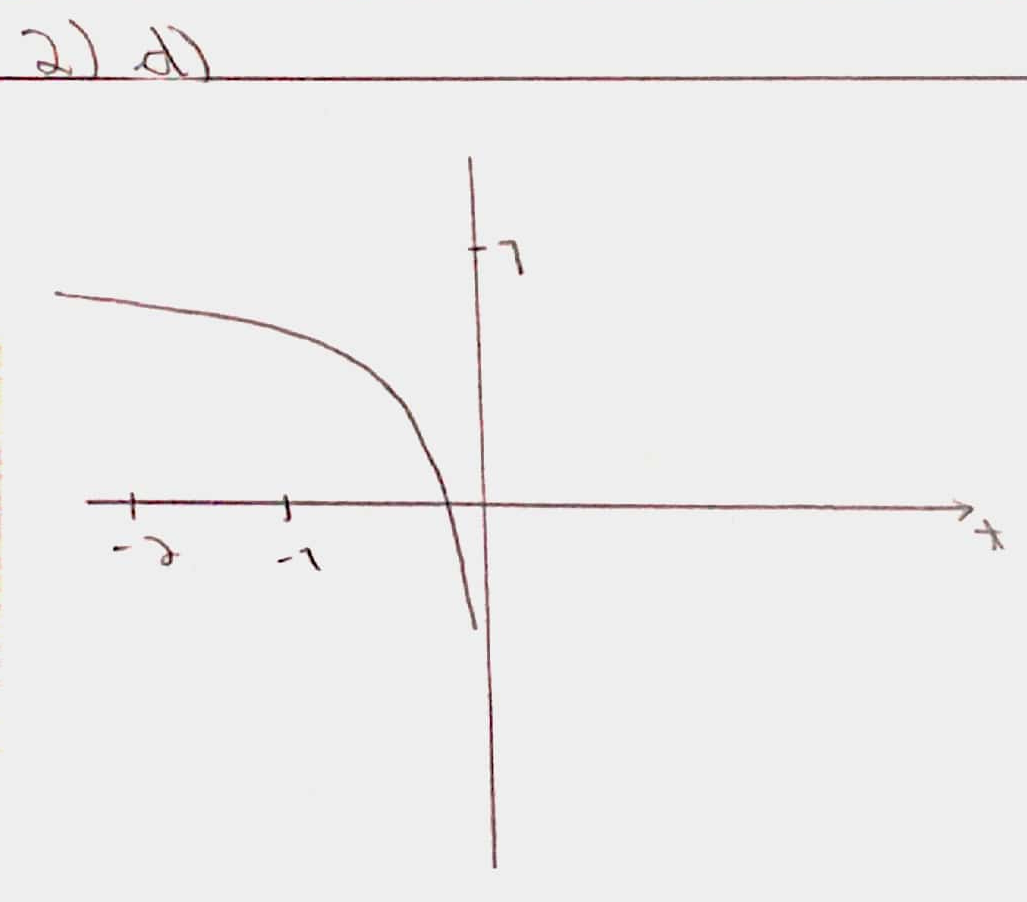
\includegraphics[scale=0.25]{Q2_d.png}
    \centering
    \caption{Esboço do gráfico - Questão 2) d)}
\end{figure}

\textbf{(e)} traçar com precisão um único gráfico com as 3 respostas ao degrau;

\begin{figure}[h]
    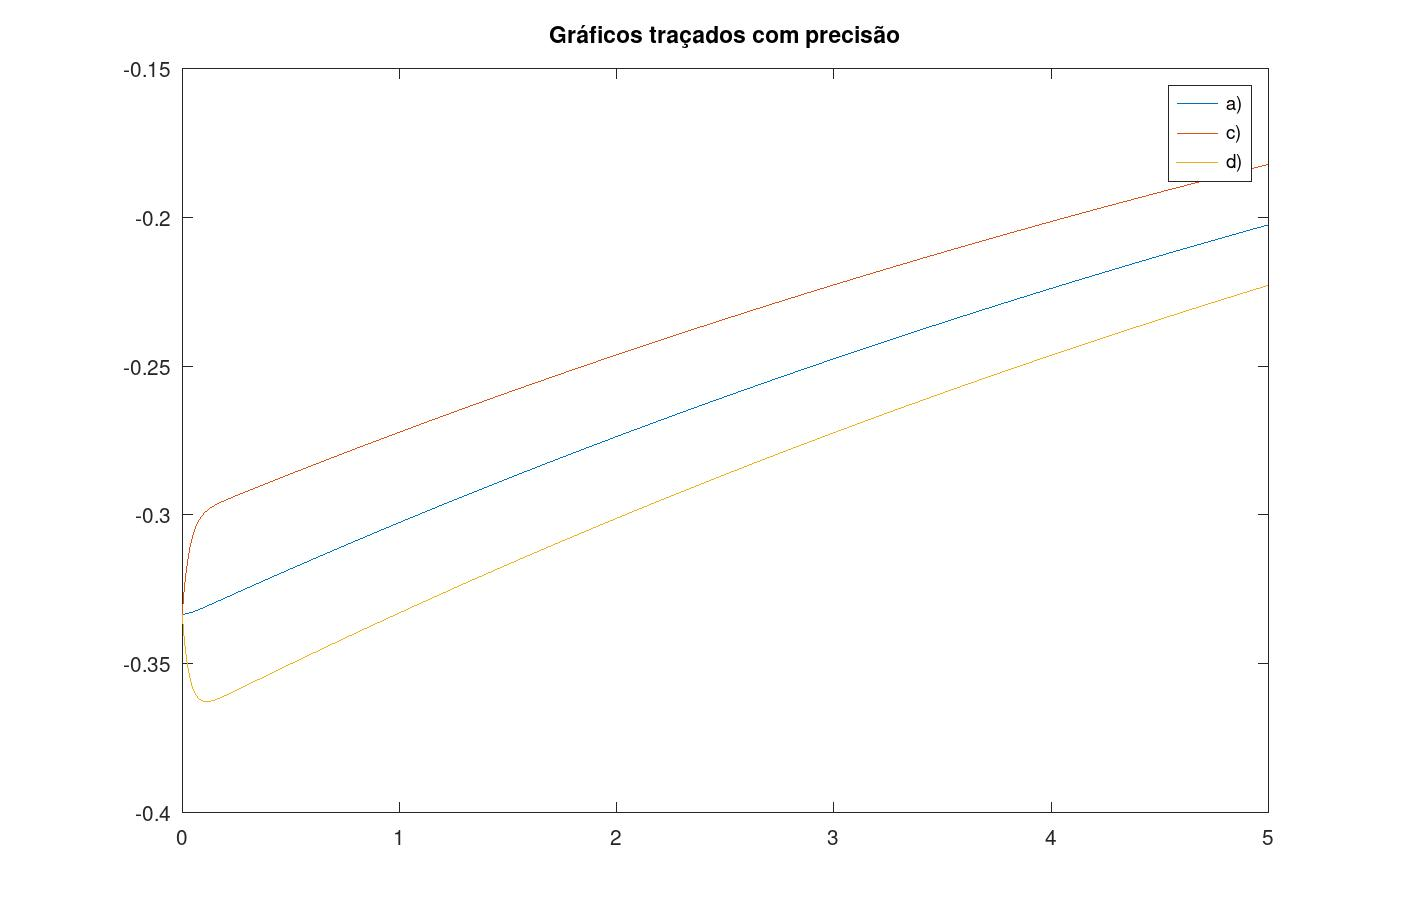
\includegraphics[scale=0.25]{plot2e}
    \centering
    \caption{Gráficos da questão 2) e)}
\end{figure}

\textbf{(f)} calcular a resposta a seno $u(t) = \sen(\omega t)$ para $b_1 = 0, \omega = 4a_0$ e esboçar o seu gráfico.

Aqui, teremos a seguinte EDO:

\[\ddot{y}(t) + 30\dot{y}(t) + 3y(t) = \sen(12t)\]

Como $y(0^-) = 0$, pois o sistema é relaxado, fazendo a transformada de Laplace em ambos os lados, teremos:

\[s^2Y(s) + 30sY(s) + 3Y(s) = \frac{12}{s^2 + 144}\]
\[Y(s)\left[s^2 + 30s + 3\right] = \frac{12}{s^2 + 144}\]
\[Y(s) = \frac{1}{s^2 + 30s + 3} \cdot \frac{12}{s^2 + 144}\]

Podemos fazer, primeiramente, a separação entre os dois produtos principais, de forma que fique como abaixo:

\[\frac{1}{s^2 + 30s + 3} - \frac{1}{s^2 + 144}\]

Corrigindo a equação acima, multiplicamos por um fator, tendo:

\[Y(s) = \frac{12}{141 - 30s} \cdot \left[\frac{1}{s^2 + 30s + 3} - \frac{1}{s^2 + 144}\right]\]

Fazendo por partes, podemos começar a separar a primeira parcela $\frac{1}{s^2 + 30s + 3}$.

\[\frac{1}{s^2 + 30s + 3} = \frac{1}{2\sqrt{222}} \cdot \left[ \frac{1}{s + 15 - \sqrt{222}} - \frac{1}{s + 15 - \sqrt{222}}\right]\]

E agora, a segunda parcela $\frac{1}{s^2 + 144}$.

\[\frac{1}{s^2 + 144} = \frac{1}{24j} \cdot \left[\frac{1}{s - 12j} - \frac{1}{s + 12j}\right]\]

Por partes, novamente, multiplicamos os resultados por $\frac{12}{141 - 30s}$. Começando da primeira parcela, já separada.

\[\frac{12}{141 - 30s} \cdot \left(\frac{1}{2\sqrt{222}} \cdot \left[
    \frac{1}{s + 15 - \sqrt{222}} - \frac{1}{s + 15 - \sqrt{222}}
\right]\right)\]

\[\frac{6}{\sqrt{222}} \cdot \left[ 
    \frac{1}{141 - 30s} \cdot \frac{1}{s + 15 - \sqrt{222}} - 
    \frac{1}{141 - 30s} \cdot \frac{1}{s + 15 + \sqrt{222}}
\right]\]

\[\frac{2}{\sqrt{222}} \cdot \left[ 
    \frac{1}{197 - 10\sqrt{222}} \cdot \left(\frac{30}{141 - 30s} + \frac{1}{s + 15 - \sqrt{222}}\right) -
    \frac{1}{197 + 10\sqrt{222}} \cdot \left(\frac{30}{141 - 30s} + \frac{1}{s + 15 + \sqrt{222}}\right)
\right]\]

\[\frac{2}{\sqrt{222}} \cdot \left[ 
    \frac{1}{197 - 10\sqrt{222}} \cdot \left(-\frac{1}{s - 141/30} + \frac{1}{s + 15 - \sqrt{222}}\right) -
    \frac{1}{197 + 10\sqrt{222}} \cdot \left(-\frac{1}{s - 141/30} + \frac{1}{s + 15 + \sqrt{222}}\right)
\right]\]

\[\frac{2}{\sqrt{222}} \cdot \left[ 
    \frac{-1}{s - 141/30} \cdot \frac{20\sqrt{222}}{16609} +
    \frac{1}{197 - 10\sqrt{222}} \cdot \frac{1}{s + 15 - \sqrt{222}} -
    \frac{1}{197 + 10\sqrt{222}} \cdot \frac{1}{s + 15 + \sqrt{222}}
\right]\]

Chamando de $p_1$ a primeira parcela na qual faremos a inversa de Laplace, teremos:

\[p_1(t) = 
    -\frac{40}{16609} \cdot e^{\frac{141}{30}t} +
    \frac{2}{197\sqrt{222} - 2220} \cdot e^{(-15 + \sqrt{222})t} - 
    \frac{2}{197\sqrt{222} + 2220} \cdot e^{(-15 - \sqrt{222})t}
\]

Podemos, agora, tratar da segunda parcela, também já separada. Ao final ficamos com:

\[- \frac{12}{141 - 30s} \cdot \frac{1}{s^2 + 144} = 
    -\frac{1}{2j} \cdot \left[
        \frac{30}{141 - 30s} \cdot \frac{80j}{16609} +
        \frac{1}{141 - 360j} \cdot \frac{1}{s - 12j} -
        \frac{1}{141 + 360j} \cdot \frac{1}{s + 12j}
    \right]
\]

\[ \left[
        \frac{1}{s - 141/30} \cdot \frac{40}{16609} -
        \frac{1}{282j + 720} \cdot \frac{1}{s - 12j} +
        \frac{1}{282j - 720} \cdot \frac{1}{s + 12j}
    \right]
\]

Chamando de $p_2$ a inversa de Laplace desta segunda parcela, teremos:

\[ p_2(t) = 
    \frac{40}{16609} \cdot e^{\frac{141}{30}t} -
    \frac{1}{282j + 720} \cdot e^{j12t} +
    \frac{1}{282j - 720} \cdot e^{-j12t}
\]

Somando $p_1(t) + p_2(t) = y(t)$, temos:

\[y(t) = 
\frac{2}{197\sqrt{222} - 2220} \cdot e^{(-15 + \sqrt{222})t} -
\frac{2}{197\sqrt{222} + 2220} \cdot e^{(-15 - \sqrt{222})t} -
\frac{1}{282j + 720} \cdot e^{j12t} +
\frac{1}{282j - 720} \cdot e^{-j12t}
\]

Fazendo mais alterações, chegamos em:

\[y(t) = 
\frac{2}{197\sqrt{222} - 2220} \cdot e^{(-15 + \sqrt{222})t} -
\frac{2}{197\sqrt{222} + 2220} \cdot e^{(-15 - \sqrt{222})t} -
\frac{40}{16609}\cos(12t) - \frac{47}{49827}\sen(12t)
\]

Esboçando o gráfico:

\begin{figure}[h]
    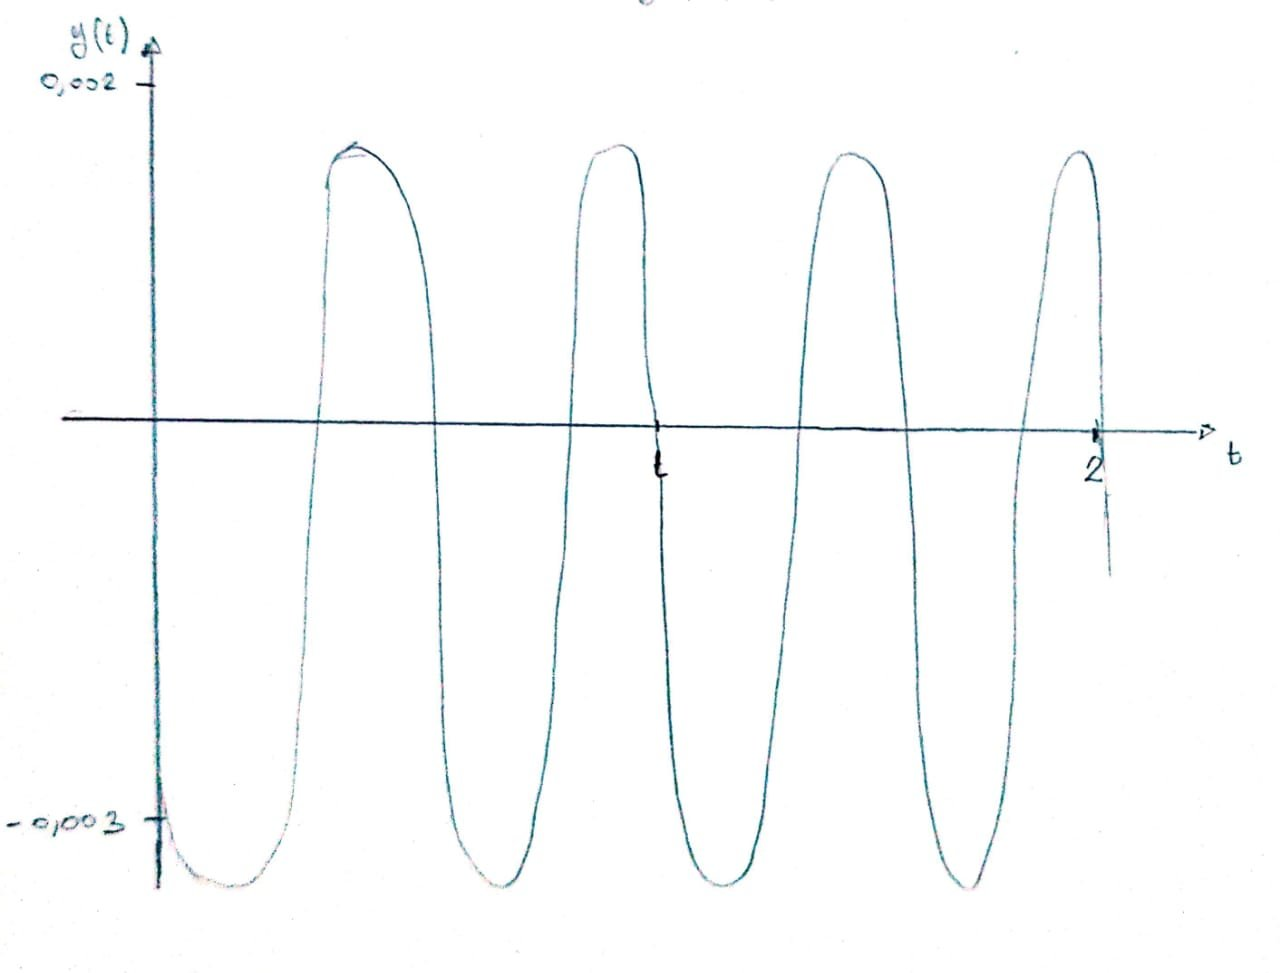
\includegraphics[scale=0.25]{plot2f}
    \centering
    \caption{Esboço do gráfico - Questão 2) f)}
\end{figure}

\vspace{\baselineskip}

\textbf{3.)} Um SLIT relaxado é descrito por uma função de transferência com numerador e denominador dados por $n(s) = K$ e $d(s) = (s + p_1)(s + p_2)(s + p_3)$.
\textbf{G2:} $p_1 = 1, p_2 = 3, p_3 = 4$

\textbf{(a)} Esboçar a resposta ao degrau unitário (escolha o valor de $K$);

A partir da equação dada no enunciado, temos:

\[ Y(s) = \frac{K}{(s+p_{1})(s+p_{2})(s+p_{3})} \cdot U(s) + G_{i}(s) \]

\vspace{\baselineskip}

Como o SLIT é relaxado, o termo $ G_{i}(s) $ é nulo.
Já o termo $ U(s) $ será $ \frac{1}{s} $, pois representa a resposta ao degrau unitário.
Além disso, vamos escolher $ K = 6 $.

Substituindo os valores na equação abaixo:

\[ Y(s) = \frac{1}{s} \cdot \frac{6}{(s+1)(s+3)(s+4)} \]

Devemos separar a equação acima em uma soma de frações parciais:

\[ Y(s) = \frac{r_1}{s} + \frac{r_2}{s+1} + \frac{r_3}{s+3} + \frac{r_4}{s+4} \]

O cálculo dos resíduos é simples, portanto será omitido. Os leitores interessados
facilmente verificarão a validade dos resultados ao lado. $ r_1 = \frac{1}{2}; \ r_2 = -1; \ r_3 = 1; \ r_4 = - \frac{1}{2}; $

$\\$
Substituindo novamente:

\[ Y(s) = \frac{1}{2s} - \frac{1}{s+1} + \frac{1}{s+3} - \frac{1}{2(s+4)} \]

Para encontrar a expressão final no domínio do tempo, deve-se aplicar a transformada inversa de Laplace:

\[ \mathcal{L}^{-1} \left\{ Y(s) \right\} = \mathcal{L}^{-1} \left\{ \frac{1}{2s} - \frac{1}{s+1} + \frac{1}{s+3} - \frac{1}{2(s+4)} \right\} \]

\vspace{\baselineskip}

Ao aplicar simples propriedades de derivação, chegamos ao resultado final:

\[ y(t) = 1(t) \cdot \left[ \frac{1}{2} - e^{-t} + e^{-3t} - \frac{1}{2} e^{-4t} \right] \]

\vspace{\baselineskip}

\textbf{(b)} esboçar a resposta ao degrau unitário quando os $p_i$ são divididos por 5;

Mantendo o mesmo valor de K, será necessário recalcular os resíduos para esse caso.

\[ Y(s) = \frac{1}{s} \cdot \frac{6}{(s+ \frac{1}{5})(s+ \frac{3}{5})(s+ \frac{4}{5})} \]

\[ Y(s) = \frac{r_1}{s} + \frac{r_2}{s+ \frac{1}{5}} + \frac{r_3}{s+ \frac{3}{5}} + \frac{r_4}{s+ \frac{4}{5}} \]

Resíduos encontrados: $ r_1 = \frac{125}{2}; \ r_2 = -125; \ r_3 = 125; \ r_4 = - \frac{125}{2}; $

\[ Y(s) = \frac{125}{2s} - \frac{125}{s+ \frac{1}{5}} + \frac{125}{s+ \frac{3}{5}} - \frac{125}{2(s+ \frac{4}{5})} \]

Resolvendo pela transformada inversa de Laplace:

\[ y(t) = 1(t) \cdot \left[ \frac{125}{2} - 125e^{-t/5} + 125e^{-3t/5} - \frac{125}{2} e^{-4t/5} \right] \]


\vspace{\baselineskip}

\textbf{(c)} esboçar a resposta ao degrau unitário quando os $p_i$ são multiplicados por 5;

\[ Y(s) = \frac{1}{s} \cdot \frac{6}{(s+5)(s+15)(s+20)} \]

\[ Y(s) = \frac{r_1}{s} + \frac{r_2}{s+5} + \frac{r_3}{s+15} + \frac{r_4}{s+20} \]

\vspace{\baselineskip}

Os resíduos são: $ r_1 = \frac{1}{250}; \ r_2 = - \frac{1}{125}; \ r_3 = \frac{1}{125}; \ r_4 = - \frac{1}{250}; $

\[ Y(s) = \frac{1}{250s} - \frac{1}{125(s+5)} + \frac{1}{125(s+15)} - \frac{1}{250(s+20)} \]

\vspace{\baselineskip}

Finalmente:

\[ y(t) = 1(t) \cdot \left[ \frac{1}{250} - \frac{1}{125}e^{-5t} + \frac{1}{125}e^{-15t} - \frac{1}{250}e^{-20t} \right] \]

\vspace{\baselineskip}

\textbf{(d)} comentar os resultados acima;

\vspace{\baselineskip}
É interessante observar que os resíduos aparecem como os coeficientes das exponenciais em cada equação, 
e as exponenciais estão associadas aos termos $ p_i $ do enunciado.

$\\$
Vamos analisar a equação final da letra a) por exemplo:

\[ y(t) = 1(t) \cdot \left[ \frac{1}{2} - e^{-t} + e^{-3t} - \frac{1}{2} e^{-4t} \right] \]

Observe que o termo $ \frac{1}{2} $ parece não ter uma exponencial associada, mas na verdade,
podemos reescrever como:

\[ y(t) = 1(t) \cdot \left[ \frac{1}{2}e^{0t} - e^{-t} + e^{-3t} - \frac{1}{2} e^{-4t} \right] \]

Através da análise acima, concluimos que o termo isolado $ \frac{1}{s} $ é na verdade: $ \frac{1}{(s+0)} $.
Assim, torna-se explícito um possível termo $ p_i $, tal que $ p_0 = 0 $

\vspace{\baselineskip}

Isso prova que os termos $ p_i $ e os resíduos encontrados em cada caso podem ser escritos da seguinte forma:

\[ y(t) = 1(t) \cdot \left[ r_1 e^{-p_0 t} + r_2 e^{-p_1 t} + r_3 e^{-p_2 t} + r_4 e^{-p_3 t} \right]\]

\vspace{\baselineskip}

\textbf{(e)} esboçar a resposta ao degrau unitário quando dois $p_i$ são multiplicados por 5 e o outro é dividido por 5;

Vamos então definir a equação da seguinte forma:

\[ Y(s) = \frac{1}{s} \cdot \frac{6}{(s+5)(s+15)(s+ \frac{4}{5})} \]

Separando em frações parciais:

\[ Y(s) = \frac{r_1}{s} + \frac{r_2}{s+5} + \frac{r_3}{s+15} + \frac{r_4}{s+ \frac{4}{5}} \]

\vspace{\baselineskip}

Resíduos: $ r_1 = \frac{1}{10}; \ r_2 = \frac{1}{35}; \ r_3 = - \frac{1}{355}; \ r_4 = - \frac{125}{994}; $

\[ Y(s) = \frac{1}{10s} + \frac{1}{35(s+5)} - \frac{1}{355(s+15)} - \frac{125}{994(s+ \frac{4}{5})} \]

Por fim:

\[ y(t) = 1(t) \cdot \left[ \frac{1}{10} + \frac{1}{35}e^{-5t} - \frac{1}{355}e^{-15t} - \frac{125}{994}e^{-4t/5} \right] \]

\vspace{\baselineskip}

\textbf{(f)} comentar os resultados acima.

\vspace{\baselineskip}

O mesmo padrão, visto nas questões anteriores, se repete aqui. 
Para cada resíduo calculado e cada termo $ p_i $, podemos expressar o resultado final 
no mesmo formato visto na questão d)

\[ y(t) = 1(t) \cdot \left[ r_1 e^{-p_0 t} + r_2 e^{-p_1 t} + r_3 e^{-p_2 t} + r_4 e^{-p_3 t} \right]\]

\end{document}